\documentclass{article}
\usepackage{exercise}
\usepackage[obeyspaces]{url}
\usepackage[dvipsnames]{xcolor}
\usepackage{graphicx}
\usepackage{listings}
\usepackage[scaled]{helvet}
\usepackage{amsmath,amssymb,amsfonts,mathtools,cancel}

% typeset in helvetica
\renewcommand*\familydefault{\sfdefault} 

\newcommand{\ipi}{i-PI}
\newcommand{\hints}[1]{\emph{Hints: #1}}
\newcommand{\lstinxml}{\lstinline[language=XML]}
\newcommand{\lstinbash}{\lstinline[language=Bash]}
\usepackage[space=true]{accsupp}

\newcommand{\pdfactualhex}[3]{\newcommand{#1}{%
\BeginAccSupp{method=hex,ActualText=#2}#3\EndAccSupp{}}}

% PASTABLE lstlisting code
\pdfactualhex{\pdfactualdspace}{2020}{\textperiodcentered\textperiodcentered}
\pdfactualhex{\pdfactualsquote}{27}{'}
\pdfactualhex{\pdfactualbtick}{60}{`}

\lstset{tabsize=4,basicstyle=\ttfamily,breaklines=true,columns=flexible,emptylines=10000}
\lstset{literate={'}{\pdfactualsquote}1
                 {`}{\pdfactualbtick}1
                 {\ \ }{\pdfactualdspace}2
}

\lstset{
    basicstyle=\ttfamily,
    keywordstyle=\color{BrickRed},
    commentstyle=\color{Gray},
    stringstyle=\color{black},
    emphstyle=\color{RedOrange},
    columns=flexible,
    showstringspaces=false,
    xleftmargin=1em,
    deletekeywords={bin,all}
}


\lstdefinelanguage{Bash}
{
   alsodigit={-,.},
   morekeywords={ cp2k.popt, lmp_ubuntu, i-pi, vmd, for, done, python, mpirun, touch, tail, trajworks, autocorr, awk, i-pi-mergebeadspdb, grep, head, cp, cd, cat, ls, pwd, bash, sed, mkdir, vi, sh}
   %morecomment=[s][\color{orange}]{#}{\}
}

%\lstdefinelanguage{Python}
%{
%    morecomment=[s][\color{orange}]{#}{\}
%}


\lstdefinelanguage{XML}
{
  morestring=[b][\color{RedOrange}]",
%  morestring=[s]{>}{<},
  morecomment=[s]{<?}{?>},
  morecomment=[s][\color{orange}]{<!--}{-->},
  identifierstyle=\color{BlueViolet},
  keywordstyle=\color{ForestGreen},
  stringstyle=\color{RedOrange},
%  tagstyle=\color{Blue},
  morekeywords={xmlns,version,type, mode, units, forcefield, filename, stride, overwrite, nbeads,prefix}% list your attributes here
}

\lstdefinestyle{XML}
{
\tagstyle=\color{Blue}
}

\title{Path integral approximations to real time correlations}
\author{Mariana Rossi}
\date{May 2016}

\begin{document}

\maketitle

\begin{figure*}[ht]
\centering
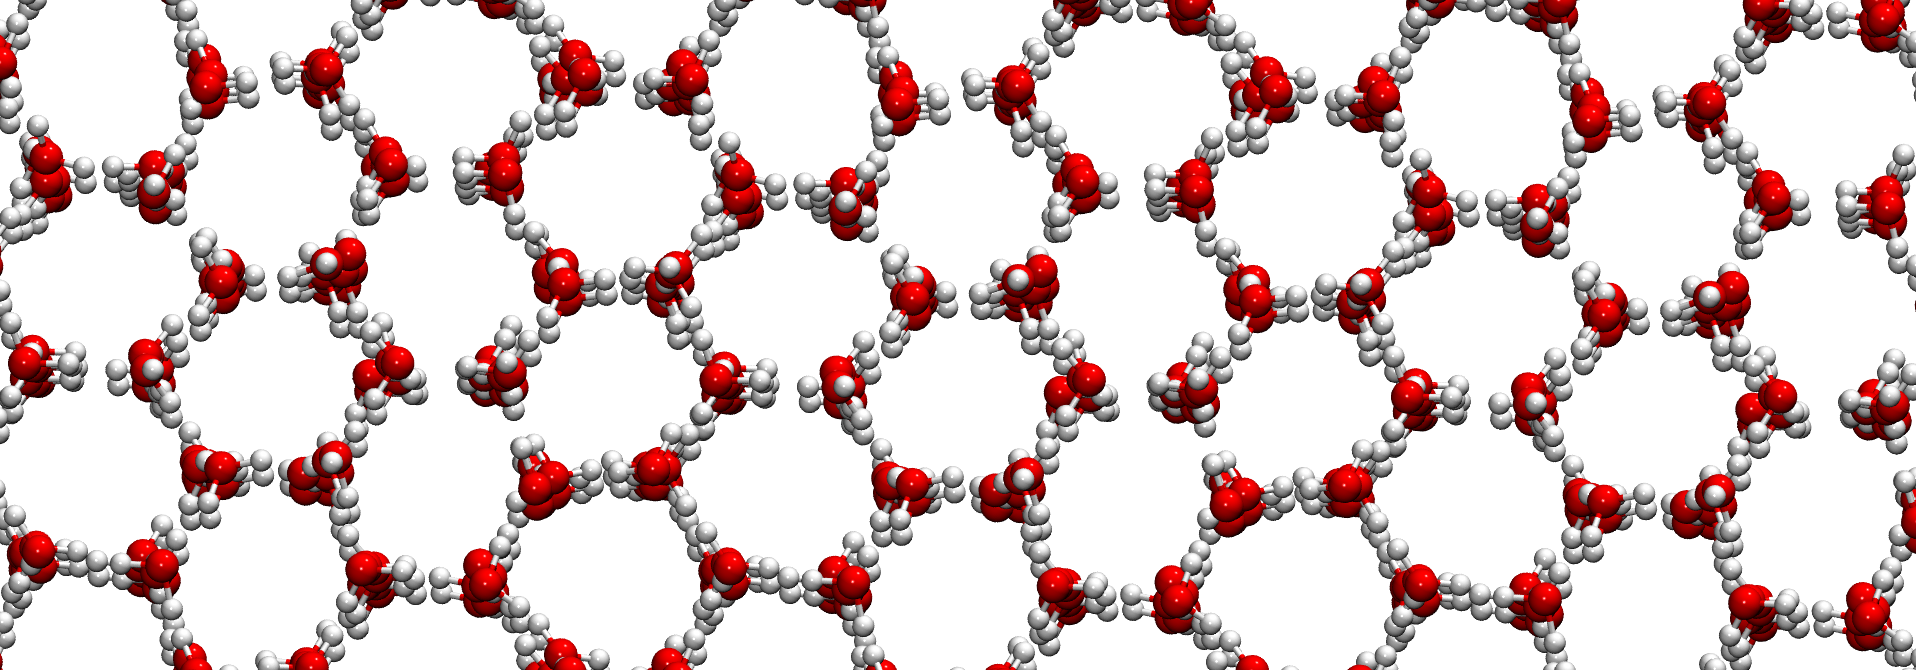
\includegraphics[width=\textwidth]{ice.png}
\end{figure*}

In this exercise we will perform
simulations of Ice Ih at 200 K,
using a simple empirical force field model based
on TIP4P-like point charges {\bf CHANGE FOR MBPOL?}. We will use this model to look
at different path integral approximations to real time correlations, calculate imaginary
time correlations from PI, and look at the relationship between them. The ice box contains 96 water molecules.
All files necessary for the exercises below can be found in the \texttt{day-3} folder.

%One can overcome some of these drawbacks by performing a Molecular Dynamics simulation of the system in question. In the framework of Linear Response Theory, one can rewrite the Fermi Golden rule by means of the Fourier transform of the dipole moment time correlation function \cite{gaigeot}:

%\begin{equation}
%I(\omega) = F(\omega) \int_{-\infty}^{\infty} dt \, \text{e}^{i\omega t} \langle  \textrm{Tr}[\exp(-\beta \hat{H}) \hat{M}(0) \hat{M}(t)] \rangle_{t_0}
%\label{dipole-dipole}
%\end{equation}

%The angular brackets denote a statistical time average for the auto-correlation of the dipole moment of the molecule.
%What our simulations actually approximate is Kubo-transformed autocorrelation functions, defined by:

%\begin{equation}
%\tilde{c}_{MM} = \frac{1}{\beta Z} \int_0^{\beta} d\lambda \textrm{Tr}\left\{  \exp[-(\beta-\lambda) \hat{H}] \hat{M}(0) \exp[-\lambda \hat{H} ]\hat{M}(t) \right\} \label{eq:autocorr-kubo},
%\end{equation}


%The relation between the Fourier transform of the canonical autocorrelation function and the Kubo-transformer one gives rise to the factor $F(\omega)$, which is proportional to $\omega^2$ (see lecture for more details).
%Eq. \ref{dipole-dipole} will give all frequencies that are active in the IR range. Therefore, the whole IR spectrum of the molecule can be calculated within one MD run, since one can choose various t=0 to average the dipole auto-correlation over.

%Usually, one approximates the autocorrelation function by the one coming from a classical (AI)MD simulation, such that only classical anharmonicities are included.
%Within the path integral formalism, approximating these autocorrelation functions calls for the development of new approximate theories, since the time dependent information is not directly accessible in PIMD. Here we will use thermostated ring polymer molecular dynamics method (TRPMD) (see Ref. \cite{trpmd}). As will be seen in the exercise, although this method can capture quantum anharmonicities to a good extent, it cannot capture explicitly coherent 
%
%A similar relation can be found for the time average of the velocity auto correlation function:
%
%\begin{equation}
%\text{VDOS}(\omega) = \sum_{i=1,N}\int_{-\infty}^{\infty} dt \, \text{e}^{i\omega t} \langle \vec{v}_i(t) \cdot \vec{v}_i(0) \rangle_{t_0}
%\label{velocity-velocity}
%\end{equation}
%


\begin{Exercise}[label={realtime},title={Velocity and dipole real time correlation functions}]

In this first exercise, we will calculate time correlation functions with path integral based methods, namely centroid molecular dynamics (CMD)~\cite{cao-voth94jcp}, ring polymer molecular dynamics (RPMD)~\cite{crai-mano04jcp}, and thermostated ring polymer molecular dynamics (TRPMD)\cite{ross+14jcp}. All these methods have been explained in the lectures, and we encourage you to look at the respective references in case you are interested in more details. We note that for the TIP4P-style of charges, the dipole moment is a linear function of the coordinates, and therefore the dipole estimator in CMD, RPMD, and TRPMD is always the same and can be calculated from the centroid positions (or velocities, in the case of its derivative). Due to time constraints we will only perform short (10 ps) simulations, and you'll be provided extensive outputs for further analysis in the exercises that require it. Inputs for simulating different PI-based methods are also provided.

\begin{itemize}

\item \textbf{Vibrational spectra with classical nuclei (Time: 10 minutes)} \\
We will start by calculating both dipole and velocity correlation functions with classical nuclei. In order to do that, we have provided pre-computed i-PI checkpoint files from a long thermalization run of Ice Ih at 200 K. Checkpoint files are a feature of i-PI that can be written through the keyword \lstinxml$<checkpoint>$ in the \lstinxml$<output>$ block of i-PI's input file, for which a syntax example would be:
    
\begin{lstlisting}[language=XML]
<checkpoint filename="restart" stride="2000" overwrite="false" />
\end{lstlisting}

    Inserting this keyword in a thermalization run provides a series of files that can be used to restart simulations from different points of the thermalization simulation (defined by the option \texttt{stride}). You can find checkpoint files from an NVT run with classical nuclei in the \texttt{ex-1/checkpoint-nvt} directory. 
    
    In order to run the NVE trajectory needed to compute the correlation functions do:
    
\begin{lstlisting}[language=Bash,emph={\$}]
$ cd ex-1/nve
$ vi nve.xml
\end{lstlisting}

   The file \texttt{nve.xml} is an example of input for NVE simulations. Take some time reading through it. For the current simulation, the most important quantity we will print out is the velocity of the atoms (here given by the centroid velocities since there is only one bead). You will notice that there are some fields marked with \texttt{xxx} in the input file. These should be {\it substituted by a number of your choice}, corresponding to the number of the checkpoint file you want to choose. You can substitute the number by hand or use a command. For example, in order to create a new directory with all necessary input files, run:

\begin{lstlisting}[language=Bash,emph={\$}]
$ number=6
$ mkdir dir_${number} 
$ sed "s/xxx/${number}/g" nve.xml > dir_${number}/input.xml
$ cd dir_${number}
$ cp ../../lammps_inputs/* .

\end{lstlisting}

Now the directory \texttt{dir\_\$number} contains all input files necessary to start our simulation. In order to launch one instance of i-PI and LAMMPS, run:

\begin{lstlisting}[language=Bash,emph={\$}]
$ i-pi input.xml &> log.ipi &
$ what=$(grep addr input.xml | sed "s/.*<address>//; s/<\/address>//")
$ sed "s/addr/$what/" in.tip4pf | lmp_ubuntu &> log.lammps &

\end{lstlisting}

The two last lines are there so as to inform LAMMPS (by changing its input), the address of the UNIX socket that is currently used by the i-PI server.

After approximately 10 minutes this simulation should be done and you can analyze the outputs. {\it Immediately after this simulation ends, launch the TRPMD simulation on the second item below before analyzing the outputs, so that it starts running in the background}.

Look at outputs using \texttt{gnuplot} and \texttt{vmd}. In order to create the dipole and velocity autocorrelations, we provide scripts in the \texttt{day-3/tools} folder that uses \lstinbash$trajworks$ functionalities in order to perform fourier transforms and calculate auto correlation functions, called \lstinbash$post-vel$ and \lstinbash$post-dpl$. We will actually calculate the dipole derivative auto correlation function, which already includes the $\omega^2$ factor that appears when relating the Kubo transform of the autocorrelation function to the standard canonical one.

Copy files to the folder where you performed the simulation and run the following commands:

\begin{lstlisting}[language=Bash,emph={\$}]
$ cp ../../../tools/post* .
$ cp ../../../tools/charges.tip4pf .
$ sh post-dpl
$ sh post-vel
\end{lstlisting}

Visualize (either with \texttt{xmgrace} or \texttt{gnuplot}) the files \texttt{dpl.ft} (Fourier transform of the dipole auto correlation) and \texttt{vel.ft} (Fourier transform of the velocity auto correlation). 

Analyze similarities and differences between them (remember this is a short simulation that cannot yield very converged correlation functions). In the folder \texttt{ex-1/precomputed-trajectories/nve/} you will find several longer precomputed and preanalyzed trajectories.


\item {\bf Vibrational spectra with quantum nuclei (Time: 1 hour)} \\
Due to time constrains, we will only perform one TRPMD run with 48 beads.
This simulation takes around one hour. For RPMD, more simulations would be needed for a reasonable spectra due to its poor ergodicity, and for (partially adiabatic) CMD, due to the much smaller time step required, the simulation would take 10 times longer.

The input file for this simulation will be in the \texttt{ex-1/trpmd} folder. The checkpoints from a PIMD simulation that we will use to start the TRPMD one can be found in \texttt{ex-1/checkpoint-pimd}. The set of bash commands you will need to launch this simulation are the following (you can change the variable \texttt{number}):

\begin{lstlisting}[language=Bash,emph={\$}]
$ cd ex-1/trpmd
$ number=6
$ mkdir dir_${number} 
$ sed "s/xxx/${number}/g" trpmd.xml > dir_${number}/input.xml
$ cd dir_${number}
$ cp ../../lammps_inputs/* .
$ i-pi input.xml &> log.ipi &
$ what=$(grep addr input.xml | sed "s/.*<address>//; s/<\/address>//")
$ for i in `seq 1 8`; do sed "s/addr/$what/" in.tip4pf | lammps &> log.$i & done
\end{lstlisting}


Beyond the velocities, here we will print out also the positions and forces on each bead, which is necessary to build the imaginary time correlation functions that we will look at in Exercise 2.

Again after the simulation is done, from the simulation directory run:

\begin{lstlisting}[language=Bash,emph={\$}]
$ cp ../../../tools/post* .
$ cp ../../../tools/charges.tip4pf .
$ sh post-dpl
$ sh post-vel
\end{lstlisting}

Visualize (either with \texttt{xmgrace} or \texttt{gnuplot}) the files \texttt{dpl.ft} and \texttt{vel.ft} and compare them with their classical counterparts that were calculated in the previous item. Which differences do you observe?

In the directories \texttt{ex-1/precomputed-trajectories/rpmd/}, \\ \texttt{ex-1/precomputed-trajectories/trpmd/}, and \\ \texttt{ex-1/precomputed-trajectories/cmd/} you'll find many precomputed and preprocessed trajectories from each different path integral based method. 

%Use the the \texttt{post-dpl} and \texttt{post-vel} scripts in each directory and then run:
%
%\begin{lstlisting}[language=Bash,emph={\$}]
%$ post-avg rpmd
%\end{lstlisting}
%
%changing \texttt{rpmd} for \texttt{trpmd} or \texttt{cmd} depending on the directory you are. 

Visualize and compare all Fourier transformed functions of dipole and velocities (.dpl and .vv), as computed from the different methods. Can you spot the spurious resonances in RPMD and the curvature problem in CMD? And do you see that the TRPMD peaks are much broader than the classical ones? 

\end{itemize}

\end{Exercise}

\begin{Exercise}[label={imaginarytime},title={Velocity imaginary time correlation function}]

In this exercise, we will calculate an example of an imaginary time correlation function, namely the velocity-velocity imaginary time correlation. These quantities are exact withing the PI formalism and can be computed from PIMD, CMD, RPMD, and TRPMD, always yielding the same result since all these methods preserve ensemble. A direct estimator for the imaginary time correlation function on the imaginary time $i \lambda_j$, with $\lambda_j=j\beta_P\hbar$, $j=0,...,n-1$, and $\lambda_n=\lambda_0$ is

\begin{equation}
c_{vv}(i \lambda_j ) = \sum_k^N \left[ \frac{3}{\beta_P m_k} - \frac{\omega_P}{P} \sum_i^{P-1} \langle (\mathbf{q}_i^{(k)}-\mathbf{q}_{i+1}^{(k)})(\mathbf{q}_{i+j}^{(k)}-\mathbf{q}_{i+j+1}^{(k)}) \rangle\right].
\end{equation}

For hints on the derivation of the equation above, check the appendix of Ref. \cite{habe+07jcp}. This expression can be recast to a centroid virial estimator form that is


\begin{equation}
c_{vv}(i \lambda_j ) = \sum_k^N \left[ \frac{3}{\beta m_k} - \frac{1}{P m_k} \sum_i^{P-1} \left\langle (\mathbf{q}_{i+j}^{(k)}-\bar{\mathbf{q}})  \frac{dV(\mathbf{q}_i^{(k)})}{d \mathbf{q}_i^{(k)}} \right\rangle\right],
\end{equation}

\noindent where $\bar{\mathbf{q}}$ is the centroid position. This is what we will calculate from our simulation. A script to calculate this expression is available in \texttt{tools/posforce2imaginaryvv.py}. Run the following commands:

\begin{lstlisting}[language=Bash,emph={\$}]
$ cd ex-2
$ cp -r ../ex-1/trpmd/dir_* .
$ cd dir_*
$ python ../../tools/posforce2imaginaryvv.py h2o-ice-trpmd 200
\end{lstlisting}

The file generated \texttt{h2o-ice-trpmd.imvacf} contains the velocity imaginary time correlation, where in the x axis is imaginary time in units of $\lambda_j \hbar/(P \beta \hbar)$. Plot this quantity. For the temperature we are simulating, we know the imaginary time correlation function through an imaginary time slice from $0$ to $\beta \hbar = 38.2$ femtoseconds. 

A more converged imaginary time velocity correlation function is given in \\
\texttt{ex-2/precomputed-imvacf/}.

\end{Exercise}



\begin{Exercise}[label={relationship},title={Relationship between imaginary and real time correlations}]

A way to check the quality of the real time autocorrelation function approximated by the PI-based methods (like the ones calculated in Ex. \ref{realtime}) is to look at sum rules that connect the real time with the imaginary time correlations. For the velocity real and imaginary time correlations, the relationship is

\begin{eqnarray}
c_{vv}(i \lambda \hbar)=\int_0^\infty f(\lambda, \omega) \tilde{F}_{vv}(\omega) d\omega \\
f(\lambda, \omega)=\frac{\beta\hbar\omega\cosh(\beta\hbar\omega/2-\lambda\hbar\omega)}{2\pi\sinh(\beta\hbar\omega/2.)}
\end{eqnarray}

\noindent where $F_{vv}(\omega)$ is the Fourier transform of the Kubo transformed real time velocity correlation function.

In Ref. \cite{tuck08book} one can also find the expression that relates the imaginary time square displacement and the real time velocity correlation function. Ref. \cite{habe+07jcp} and references therein also point to derivations of these expressions. 

By reconstructing $c_{vv}(i \lambda \hbar)$ from the vibrational spectra obtained with either TRPMD, RPMD, or CMD, and comparing to the exact $c_{vv}(i \lambda \hbar)$ obtained in Ex. \ref{imaginarytime}, one can assess (even if indirectly) how large the errors are. 

In order to reconstruct the imaginary time correlations from real time data we provide the script \texttt{tools/get\_imacf\_from\_real.py}. The syntax is:

\begin{lstlisting}[language=Bash]
python get_imacf_from_real.py [filename] [temperature] [nbeads]
\end{lstlisting}

In the folder \texttt{ex-3/convergedspecs} you will find the files \texttt{trpmd.vel}, \texttt{rpmd.vel}, and \texttt{cmd.vel}. Type (the simulations provided here were run with 56 beads):

\begin{lstlisting}[language=Bash,emph={\$}]
$ cd ex-3/convergedspecs
$ python ../../tools/get_imacf_from_real.py trpmd.vel 200 56 > trpmd.imvacf
$ python ../../tools/get_imacf_from_real.py rpmd.vel 200 56 > rpmd.imvacf
$ python ../../tools/get_imacf_from_real.py cmd.vel 200 56 > cmd.imvacf
\end{lstlisting}

Compare all the imaginary time correlations with the one provided in \texttt{ex-2/precomputed-imvacf/}. Which method yields the most accurate imaginary time correlation function?


\end{Exercise}


\clearpage

\bibliographystyle{unsrt}
\bibliography{biblio}

%\begin{thebibliography}{50}

%\bibitem{Newton} I. Newton, {\em Philosophi\ae{} Naturalis Principia Mathematica}, London (1687)
%\bibitem{tuckerman} D. Marx, M. E. Tuckerman, J. Hutter, and M. Parrinello Nature \textbf{397}, 601 (1999)
%\bibitem{Kolafa1996} J. Kolafa,  Mol. Simul. \textbf{18}, 193 (1996)
%\bibitem{KuehneParrinello2007} K\"uhne, Thomas D. \textit{et al}., Phys. Rev. Lett. \textbf{98}, 066401 (2007)
%\bibitem{frenkel-smit} D. Frenkel and B. Smit, \textit{Understanding Molecular Simulation: from algorithms to applications}, second edition, Academic Press 2002.
%\bibitem{niklasson-challacombe} A. M. N. Niklasson, C. J. Tymczak, and M. Challacombe, Phys. Rev. Lett. \textbf{97}, 123001 (2006)
%\bibitem{arias-joannop} T. A. Arias, M. C. Payne, and J. D. Joannopoulos, Phys. Rev. B \textbf{45}, 1538 (1992)
%\bibitem{niklasson} A. M. N. Niklasson, Phys. Rev. Lett. \textbf{100}, 123004 (2008)
%\bibitem{ishida} H. Ishida \textit{et al.}, Chem. Phys. Lett. \textbf{282}, 115 (1998)
%\bibitem{andersen} H. C. Andersen, J. Chem. Phys. \textbf{72}, 2384 (1980)
%\bibitem{nosehoover} S. Nos\'{e}, J. Chem. Phys. \textbf{81}, 511 (1984). W.G. Hoover, Phys Rev. A \textbf{31}, 1695 (1985)
%\bibitem{bdp} G. Bussi, D. Donadio, and M. Parrinello, J. Chem. Phys. \textbf{126}, 014101 (2007)
%\bibitem{colored} M. Ceriotti, G. Bussi, M. Parrinello, JCTC \textbf{6}, 1170 (2010)\\ \texttt{https://epfl-cosmo.github.io/gle4md/}
%\bibitem{martyna-klein-tuckerman} G. Martyna, M. Klein, M. Tuckerman,  J. Chern. Phys. {\bf 97}, 2635 (1992)
%\bibitem{ipi} M. Ceriotti, J. More, D. E. Manolopoulos, CPC \textbf{185} 1019 (2013)
%\bibitem{Feynman} R. P. Feynman and A. R. Hibbs, \textit{Quantum Mechanics and Path Integrals}, Emended Edition, Dover (2010)
%\bibitem{trotter} H. F. Trotter, Proc. Amer. Math. Soc. {\bf 10}, 545 (1959)
%\bibitem{piglet} M. Ceriotti, D. E. Manolopoulos, PRL \textbf{109}, 100604 (2012)
%\bibitem{trpmd} M. Rossi, M. Ceriotti, D. E. Manolopoulos, JCP \textbf{140}, 234116 (2014)
%\bibitem{pile} M. Ceriotti, M. Parrinello, T. E. Markland, D. E. Manolopoulos, JCP {\bf 133}, 124104 (2010)
%\bibitem{ramirez-marx} R. Ramirez, T. Lopez-Ciudad, P. Kumar, and D. Marx, J. Chem. Phys. \textbf{121}, 3973 (2004)
%\bibitem{berendsen}H. J. C. Berendsen et al., J. Chem. Phys. \textbf{81}, 3684 (1980)
%\bibitem{gaigeot} M-P. Gaigeot, M. Martinez, and R. Vuilleumier, Mol. Phys. \textbf{105}, 2857 (2007)
% \bibitem{borysow-fromm} J. Borysow, M. Moraldi, and L. Frommhold, Molec. Phys. \textbf{56}, 913 (1985)
% \bibitem{ramirez-marx} R. Ramirez, T. Lopez-Ciudad, P. Kumar, and D. Marx, J. Chem. Phys. \textbf{121}, 3973 (2004)
% \bibitem{mcquarrie} D. McQuarrie, \textit{Statistical Mechanics}, University Science Books, 1st. ed., (2000)
% \bibitem{SKE} T. M. Gibbons and S. K. Estreicher, Phys. Rev. Lett. \textbf{102}, 255502 (2009).
% \bibitem{AsMe} N. W. Ashcroft and N. D. Mermin, {\it Solid State Physics}, Cengage Learning, (1976).
%\end{thebibliography}

\end{document}
